% =========================================================================
\chapter{Why rare days are hard: imbalanced classification}
\label{ch:imb}
% =========================================================================

\section{Class imbalance}
A data set is \textbf{imbalanced} when one class is much rarer than the other. Here the rare (\emph{minority}) class,
extreme days, is about 1\% of training rows; the common (\emph{majority}) class, normal days, is 99\%. For every
extreme row the model sees 99 normal ones.

\section{The accuracy trap}
\textbf{Accuracy} is the share of all predictions that are right. In the test years 98.06\% of days are normal, so a
``model'' that \emph{never} warns is 98\% accurate and completely useless: it catches no extreme day. That is why the
project never judges models by accuracy (Chapter~\ref{ch:metrics}).

\section{What goes wrong in training}
A classifier learns by reducing its total error. Getting all normal days right already makes the error tiny, so the
few extreme days have little influence. Within the extremes, the \emph{most severe} days are rarer still (only a few
hundred in 30 years), so they are the worst learned, although they are the most dangerous.

\section{Standard fixes, and their limits}
\begin{itemize}
  \item \textbf{Class weights:} count each extreme row as if it were many rows. Does not add new information.
  \item \textbf{Random oversampling:} repeat real extreme rows. The model may memorise them (overfitting).
  \item \textbf{SMOTE} (Synthetic Minority Over-sampling Technique): make a new rare row on the straight line between
        a real rare row and one of its nearest rare neighbours. Variants: Borderline-SMOTE (only near the class
        boundary) and ADASYN (more where the class is hard).
\end{itemize}

\begin{figure}[H]
\centering
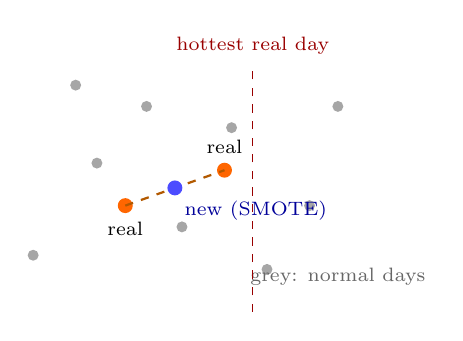
\begin{tikzpicture}[scale=0.9]
\foreach \p in {(0.3,0.5),(1.2,1.8),(2.4,0.9),(3.1,2.3),(0.9,2.9),(4.2,1.2),(3.6,0.3),(1.9,2.6),(4.6,2.6)}
  \fill[black!35] \p circle (2.2pt);
\fill[orange!80!red] (1.6,1.2) circle (3pt); \fill[orange!80!red] (3.0,1.7) circle (3pt);
\draw[dashed,orange!70!black,thick] (1.6,1.2) -- (3.0,1.7);
\fill[blue!70] (2.3,1.45) circle (3pt);
\node[font=\scriptsize,anchor=north] at (1.6,1.1) {real};
\node[font=\scriptsize,anchor=south] at (3.0,1.8) {real};
\node[font=\scriptsize,blue!60!black,anchor=north west] at (2.3,1.4) {new (SMOTE)};
\node[font=\scriptsize,black!60] at (4.6,0.2) {grey: normal days};
\draw[dashed,red!60!black] (3.4,-0.3) -- (3.4,3.2); \node[font=\scriptsize,red!60!black,anchor=south] at (3.4,3.2) {hottest real day};
\end{tikzpicture}
\caption{SMOTE places a new rare point between two real ones. It can never create a day hotter than the hottest real
one (dashed line), and it knows nothing about the physics of extremes.}
\end{figure}

\section{The idea of this project}
Instead of copying or interpolating, \textbf{learn} what extreme days look like with a \emph{generative model}
(Chapter~\ref{ch:gen}), and use \textbf{extreme value theory} (Chapter~\ref{ch:evt}) to decide how severe the new days
should be, so that most go to the thinnest, hottest part of the tail without passing what is physically possible.

\begin{sayit}
``Only 1 day in 100 is extreme, so a model that never warns is 98\% accurate and useless. Usual fixes reweight or copy
the rare days, or interpolate between them like SMOTE, which can't go beyond the hottest real day. So I generate new
extreme days instead, and let extreme value theory decide where in the tail to put them.''
\end{sayit}
